\chapter{Tecnologie e Servizi}

\section{Docker}

Docker è diventato negli anni il sistema più popolare per gestire la virtualizzazione basata su container. Può essere visto come un tipo di macchina virtuale leggera, in quanto riesce a garantire le stesse caratteristiche di quelle tradizionali, ma con un overhead minore, sia in termini di efficienza nell'esecuzione, che di spazio occupato. 

\begin{figure}[htbp]
    \centering
    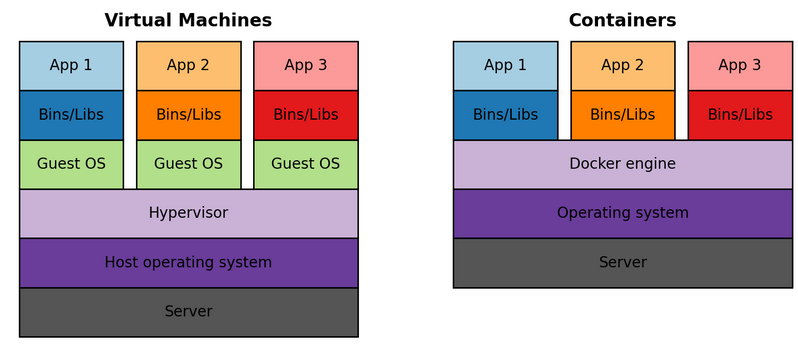
\includegraphics[width=0.9\textwidth]{figures/containers-and-vms.png}
    \caption{Confronto tra macchine virtuali tradizionali e containers.} 
    \label{fig:virt-tech}
\end{figure}

Essi vengono eseguiti direttamente sul sistema operativo dell'host, senza la necessità di chiamate di sistema multiple. Vengono impacchettate solo le librerie necessarie nell'immagine di base fornita al container. In realtà, la sua value proposition è legata alla possibilità di poter lanciare una applicazione ovunque, con la garanzia che questa funzioni sempre. L'analogia con i container nel mondo reale è diretta: quelli utilizzati nel commercio, possono essere adattati indipendentemente dall'ambiente di trasporto. Allo stesso modo l'applicazione che viene eseguita, funzionerà a prescindere dall'ambiente di esecuzione, qualsiasi sistema operativo esso sia, con l'unica limitazione sull'instruction set per cui è stata generata la build.  Nella pratica, quindi, esistono due definizioni in base all'utilizzatore di questa tecnologia: se si parla di gestione di una infrastruttura, allora l'attenzione è spostata verso la virtualizzazione, mentre se il focus è relativo alle applicazioni, allora si può vedere Docker come una tecnologia orientata alla portabilità. In generale, le macchine virtuali devono garantire un serie di proprietà per poter essere definite tali, che sono:

\begin{itemize}
	\item \textbf{consolidamento}: inizialmente, all'interno delle organizzazioni, ciascuna applicazione veniva eseguita su una macchina distinta, rendendo l'utilizzo delle risorse inefficiente. La virtualizzazione ha permesso di superare questa limitazione, con l'esecuzione di software differenti all'interno della stessa macchina.
	\item \textbf{isolamento}: questa proprietà consente ad ogni applicazione di vedere l'ambiente come se fosse una macchina a sé stante, nonostante il consolidamento. I sistemi operativi offrono funzionalità di isolamento base come l'astrazione dello spazio di indirizzamento di un processo, ma questo non è sufficiente per una applicazione self-contained. Diversi applicativi infatti possono interferire tra di loro già solo nell'utilizzo della memoria, nel caso di sovra-allocazioni, comportando un degrado delle prestazioni. Lo stesso ragionamento, a maggior ragione, si può applicare anche per la gestione della cpu, della rete e del filesystem che all'interno di un sistema operativo sono risorse completamente condivise tra processi. 
	\item \textbf{flessibilità}: il controllo dei container è molto semplice in quanto Docker prevede dei comandi standard per la loro gestione, come l'avvio, la pausa e lo stop. Gli orchestratori giocano un ruolo fondamentale per riallocare i container in nodi diversi dell'infrastruttura, per esempio in caso di manutenzione o sovraccarico. Questo processo avviene senza particolari overhead, in quanto i container, a differenza delle macchine virtuali tradizionali hanno dei tempi di attivazione molto bassi.
	\item \textbf{portabilità}: come già visto, i container possono essere avviati in qualsiasi piattaforma, indipendentemente dal sistema operativo, dall'hardware, dalle librerie necessarie e dalle loro versioni. Questo comporta un grande vantaggio anche nell'uso di linguaggi di programmazione di basso livello quando l'efficienza è fondamentale. Linguaggi come Java, ad esempio, si servono di macchine virtuali per poter garantire la portabilità del codice, ma il tempo di esecuzione aumenta notevolmente. 
\end{itemize}

L'implementazione dei container è stata possibile grazie a due elementi presenti all'interno dei sistemi operativi: namespaces e cgroups(control groups). Si tratta di features che inizialmente non erano state pensate per la virtualizzazione, ma solo nell'ottica di avere dei processi isolati. Non si è quindi arrivati subito alla definizione di container, ma ci sono state delle tappe risolutive di diversi problemi che gli sviluppatori avevano all'inizio degli anni 2000. I namespaces permettevano la gestione della visibilità relativa alle risorse per ogni processo, mentre i cgroups servivano a limitare l'utilizzo di quanto allocato. Nel secondo caso, esistevano già dei meccanismi di questo tipo all'interno del kernel Linux (e.g. cpulimit, nice), ma non erano centralizzati e potevano essere applicati solo a singoli processi. L'evoluzione dei cgroups è fondamentalmente quella di estendere il tutto ad un gruppo di task in maniera modulare, con la possibilità di definire delle gerarchie nella gestione delle risorse. Le tecnologie basate su container come Docker hanno integrato questi meccanismi nel loro layer di virtualizzazione, in modo tale da fornire delle primitive di alto livello. Infatti, sfruttando, direttamente le precedenti astrazioni, si incorre in problemi di accessibilità: solo utenti esperti, come amministratori di sistema, sarebbero in grado di maneggiare questo tipo di virtualizzazione. Oltretutto anche in questo caso gli errori sono inevitabili, a causa della complessità di gestione. 

Docker presenta infine una particolarità a livello di filesystem: rispetto alle macchine virtuali tradizionali o ai container LXC, che sfruttano un filesystem in senso stretto, questa tecnologia utilizza il concetto di Union Filesystem. 

\begin{figure}[htbp]
    \centering
    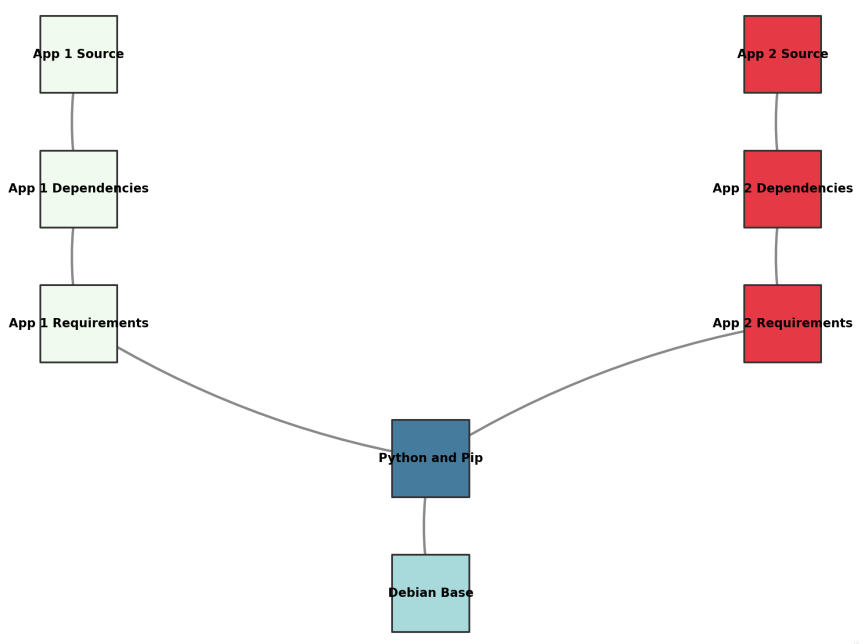
\includegraphics[width=0.69\textwidth]{figures/docker-image-layers.png}
    \caption{Esempio di condivisione di layers in Docker. Le due immagini risultanti hanno la stesso sistema di base, condividendo lo stesso ambiente (Debian) e runtime (Python).}
    \label{fig:image-layers}
\end{figure}

Si tratta di un sistema che combina diversi filesystem restituendo logicamente un'unica struttura. Nell'implementazione di Docker, lo Union Filesystem si presenta come una gerarchia di strati, tutti in sola lettura, a cui ne viene aggiunto uno scrivibile al lancio del container. Questo meccanismo, come si può vedere in Figura \ref{fig:image-layers} permette la condivisione della stessa immagine di base, evitando allo stesso tempo di dover duplicare lo spazio di memoria e che modifiche da parte di una macchina possano influenzare ciò che vedono gli altri container basati sulla stessa istanza, attuando così un primo livello di isolamento (quello più generale con l'host viene sempre implementato attraverso i namespaces). 

La realizzazione pratica di questa funzionalità è possibile grazie al concetto di copy-on-write, già utilizzato nella creazione dei processi. In questo caso il funzionamento è analogo, ma si applica a livello di memoria secondaria. Ogni modifica all'immagine di base, attraverso il layer in scrittura di più alto livello, è ciò che viene salvato. Non si apportano modifiche all'intera memoria: in pratica è un meccanismo basato sulle differenze. Una volta che si esegue il commit di un'immagine, gli strati vengono congelati e ne formano una nuova. Dal punto di vista dell'utilizzatore, questo sistema si rivela molto utile, perché si possono comporre nuove immagini impilando nuovi layer a quelli già esistenti, senza preoccuparsi di quelli sottostanti: grazie alla portabilità il loro funzionamento è automaticamente garantito. La composizione non è l'unica proprietà interessante che emerge da questa architettura, ma anche modularità, riutilizzo ed efficienza. Quest'ultima è importante sia in termini di spazio, perché come già visto i layer inferiori vengono condivisi, sia in termini di tempo. Quando si costruisce una nuova immagine, infatti, verranno aggiunti o scaricati solo gli strati di più alto livello per la generazione di quella nuova, invece di dover ri-eseguire l'operazione ogni volta per l'intero stack.
  	
\section{MQTT} %mancano definizione esplicita del protocollo, ma emergono nelle responsabilità del broker; subscribe, unsubscribe
Message Queue Telemetry Transport (MQTT) è un protocollo orientato ai messaggi, basato su TCP, il cui obiettivo è quello di fornire un meccanismo leggero, per dispositivi con risorse limitate e connessioni instabili. Il formato dei dati infatti è semplice ed è pensato per essere affidabile e fault-tolerant. Proprio per le sue caratteristiche, con il tempo è diventato uno standard nelle le applicazioni IoT, ad esempio monitoraggio remoto e raccolta di dati in industria, domotica e ambiente. MQTT si basa su un'architettura publish-subscribe. Ciò permette di disaccoppiare l'invio dei messaggi tra produttori e consumatori, attraverso un broker. Si tratta di un metodo di comunicazione indiretto, in quanto per chi pubblica non è necessario conoscere la destinazione, come invece avviene nelle architetture client-server classiche. Il funzionamento è analogo a quello delle newsletter. Quando un utente è interessato ad un certo argomento, lascia il proprio indirizzo email, in modo tale da ricevere aggiornamenti. Analogamente, in un sistema publish-subscribe, le entità che devono ricevere determinati messaggi da un publisher, si iscrivono ad un canale. 

\begin{figure}[htbp]
    \centering
    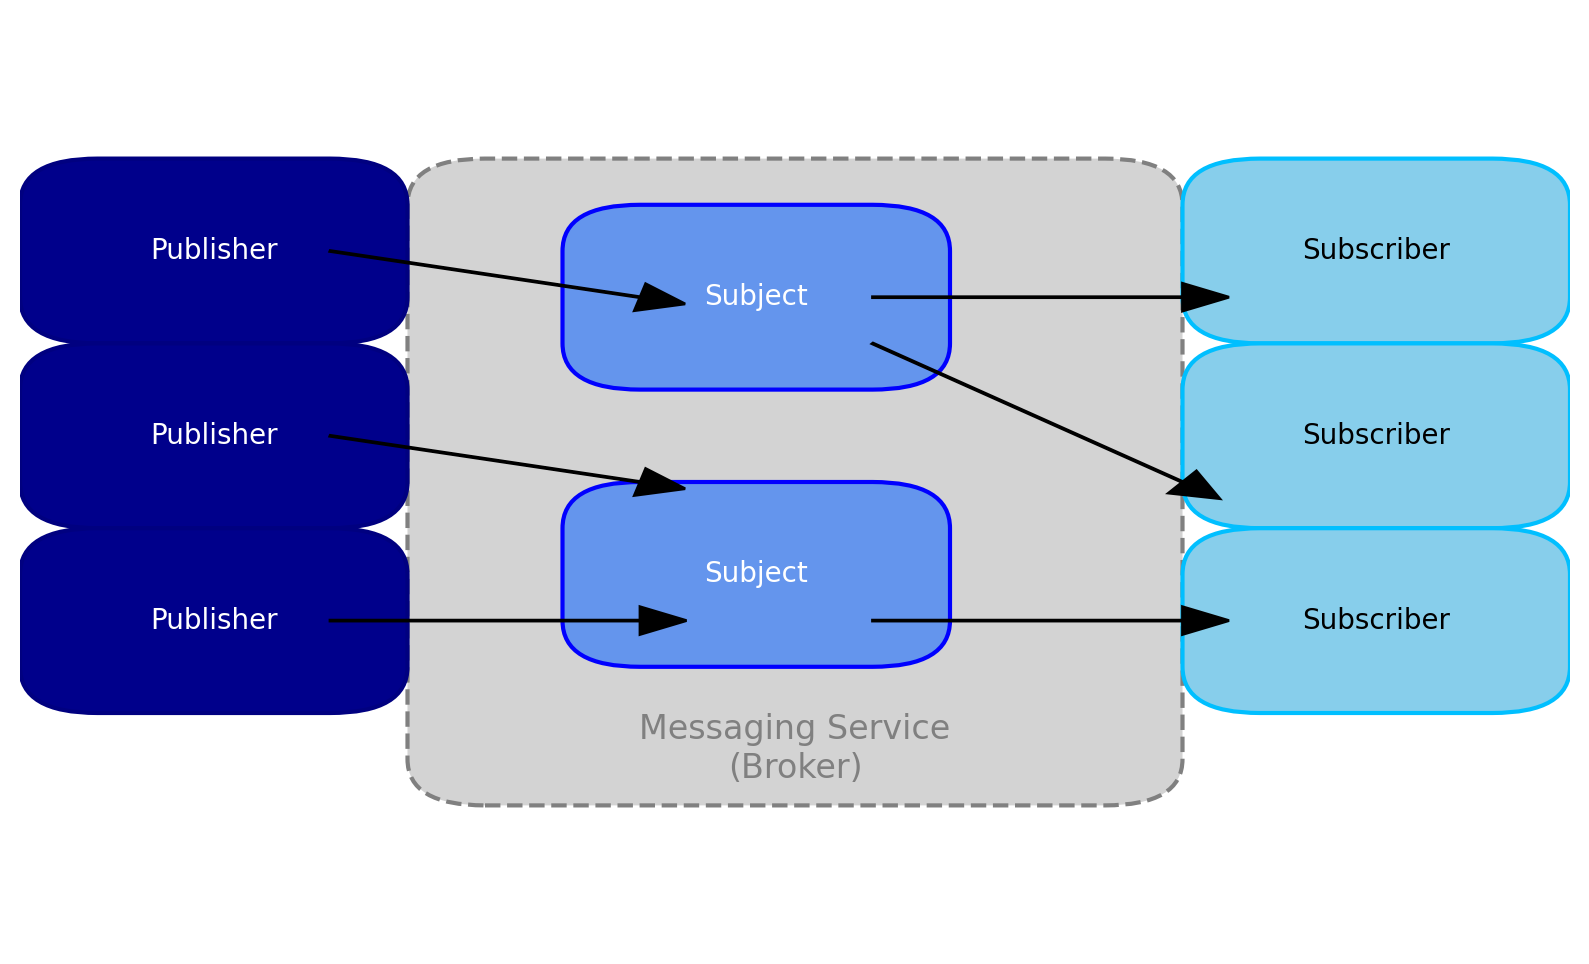
\includegraphics[width=0.7\textwidth]{figures/pub-sub-arch.png}
    \caption{Schema architettura publish-subscribe.}
    \label{fig:pub-sub}
\end{figure}

\noindent Oltre al disaccoppiamento, questo tipo di pattern fornisce ulteriori vantaggi\cite{a9IoT4Arch}. E' possibile aggiungere nuovi publisher o subscriber senza dover modificare la logica esistente, il che rende l'architettura facilmente scalabile. Si tratta di uno dei motivi per cui il cloud riesce a gestire facilmente milioni di messaggi in un breve intervallo di tempo ed avere migliaia di publishers. Inoltre, ogni parte del sistema non dipende dalle altre, favorendo la comunicazione asincrona, poiché nessun publisher deve aspettare per l'invio di nuovi messaggi prima che i consumatori finiscano. Allo stesso modo, i consumatori non devono attendere che altri ricevano i messaggi per poter proseguire con l'elaborazione delle proprie informazioni. Questo tipo di pattern viene implementato in tanti sistemi, come quelli delle notifiche push nelle applicazioni mobili, nei servizi gestiti del cloud ed infine nei sistemi IoT. In quest'ultimo caso si utilizza il protocollo MQTT, dove i canali di comunicazione vengono descritti come topic. Essi sono univocamente definiti all'interno dei broker, attraverso una struttura gerarchica, che ricorda i path nelle URI. Ad esempio, un topic può essere dichiarato come: \texttt{factory/floor/sensor1}. Non esiste un meccanismo esplicito di creazione dei topic, ma vengono specificati contestualmente alla pubblicazione di un messaggio.

Il broker ha la responsabilità di connettere, se autorizzati, i diversi client della rete, di tenere traccia dello stato di connessioni precedenti e di filtrare i dati in arrivo dai publisher. Per il discorso di efficienza previsto da questo protocollo, infatti, devono essere distribuiti solo i pacchetti necessari al funzionamento del sistema, e quindi la capacità di filtro è un elemento fondamentale. In particolare, esistono diverse tipologie di controllo delle informazioni in transito. Quello più importante è il topic filter, dove un messaggio deve contenere necessariamente un topic nell'header, e sarà compito del broker ritrasmetterlo o ignorarlo in base a come è stata implementata la sua logica. In generale i filtri vengono usati per riferirsi ad un insieme di topic, sfruttando due tipologie di wildcards. Si utilizza il segno "+" per indicare un intero livello nella gerarchia del path definito dal topic. Ad esempio \texttt{factory/+/sensor1} serve per tutti i sensor1 nei diversi piani di una fabbrica. Il secondo simbolo, cioè "\#" si riferisce ad una intera sottogerarchia nel path. \texttt{factory/\#} e \texttt{factory/first/\#} filtrano rispettivamente tutti i messaggi provenienti dal sito industriale e quelli generati dal primo piano del complesso. MQTT è un protocollo progettato con l'affidabilità in mente: in base al contesto (hardware, banda, latenza) e al tipo di applicazione, fornisce diversi livelli di Quality of Service(QoS):

\begin{itemize}
	\item \textbf{QoS0}: modalità di funzionamento default in MQTT, se non specificato. I messaggi vengono inviati con una logica fire-and-forget, senza la garanzia che il processo vada a buon fine. Il publisher o il broker inviano i pacchetti senza alcun tipo di risposta da parte di un subscriber. Non ci sono ulteriori garanzie oltre a quelle fornite dal protocollo TCP.
	\item \textbf{QoS1}: assicura che il messaggio venga inviato almeno una volta. Questo meccanismo si basa su pacchetti di acknowledgment provenienti dal ricevente, per cui se non arriva nessuna risposta, l'informazione deve essere ritrasmessa.
	\item \textbf{QoS2}: si tratta del livello di qualità di servizio più alto. Il messaggio viene inviato una sola volta, grazie ad una serie di pacchetti di controllo generati dalle entità in gioco. Può essere visto come un acknowledgement incrociato tra publisher e ricevente. Quello che avviene in più rispetto a QoS1, è l'inoltro dei pacchetti publish-realease, per indicare il rilascio del messaggio dalla memoria del publisher, e publish-complete da parte del ricevente per chiudere la comunicazione. In questo modo, alla fine del processo, l'informazione è stata inviata e gli attori in gioco sono totalmente sincronizzati dal punto di vista della ricezione.   
\end{itemize}

\begin{figure}[htbp]
    \centering
    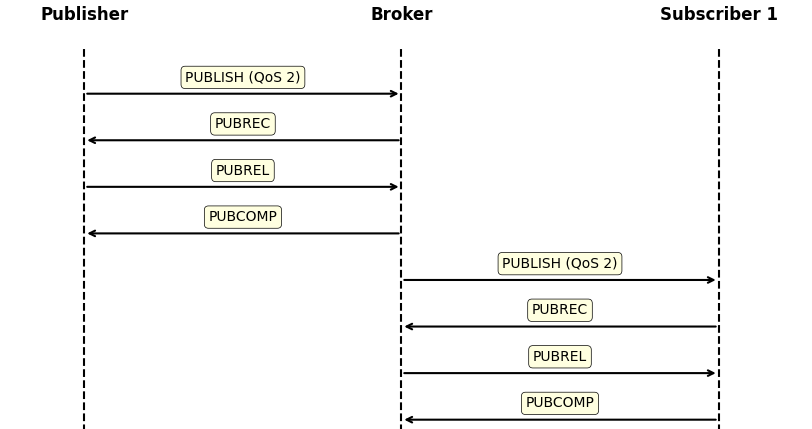
\includegraphics[width=0.85\textwidth]{figures/qos2.png}
    \caption{Flusso pacchetti di controllo per QoS2. I livelli più semplici funzionano in maniera simile, con un numero di pacchetti inferiore. Si può notare come il disaccoppiamento fornito dal broker faciliti lo scambio dei messaggi.}
    \label{fig:qos2}
\end{figure}





Il QoS viene negoziato al momento della connessione con il broker, ed in base alle sue capacità può essere dinamicamente modificato in un secondo momento. Nell'affrontare il concetto di qualità di servizio, si è visto quindi il funzionamento della publish da parte di un client, ma esistono altri tipi di operazioni in questo pattern, cioè subscribe, unsubscribe e ping. In particolare quest'ultimo risulta fondamentale per l'implementazione del Last Will and Testament(LWT), un metodo per comunicare la disconnessione di un publisher all'interno della topologia. LWT è un messaggio contente il topic, il QoS e un payload da inoltrare a tutti i subscriber che fino a quel momento ricevevano le notifiche. Questo pacchetto viene fornito nel momento in cui un client si connette per la prima volta al broker, prima che inizi l'invio effettivo dei dati per gli altri client. Se attraverso delle operazioni di ping, impostate con un certo timer, una delle due parti non riceve risposta, allora si assume esserci stata una disconnessione. A quel punto, se è il client ad essere offline, il broker invierà il Will ai subscribers. Un'ultima caratteristica importante per il funzionamento di MQTT, è la persistenza. Il broker mantiene le informazioni di sessione per i client disconnessi, in modo tale da riottenere facilmente le iscrizioni ai topic e i messaggi in coda che non avevano ricevuto (se si tratta di QoS1 e QoS2, pensati come già visto per la trasmissione affidabile). Inoltre, i publisher possono impostare un flag RETAINED nei messaggi, così da salvarli in maniera indefinita nel broker. L'obiettivo di questa funzionalità è garantire l'invio di un determinato messaggio ad un client indipendentemente dal momento della sua iscrizione.  

\section{Protocolli di streaming locale}
La rete IP è nata per la trasmissione di dati in zone geograficamente distanti tra loro. Le comunicazioni inizialmente erano basate sull'invio di file ed e-mail. La naturale estensione di questo meccanismo è stata quella di poter trasferire informazioni multimediali come animazioni, voce e video in tempo reale, il che ha comportato l'introduzione di nuovi requisiti nello stack IP. Se da un lato il protocollo di livello 3 era sufficiente per le comunicazioni più semplici, esso risultava inaffidabile sia in termini di mantenimento di informazioni, che di ordine di arrivo. L'aggiunta del livello TCP ha risolto questa limitazione, ma con l'avvento dello streaming si sono presentati nuovi problemi, legati soprattutto alla latenza e al jitter, rispettivamente il tempo totale per la trasmissione di un pacchetto e la variabilità del delay. 

\begin{figure}[htbp]
    \centering
    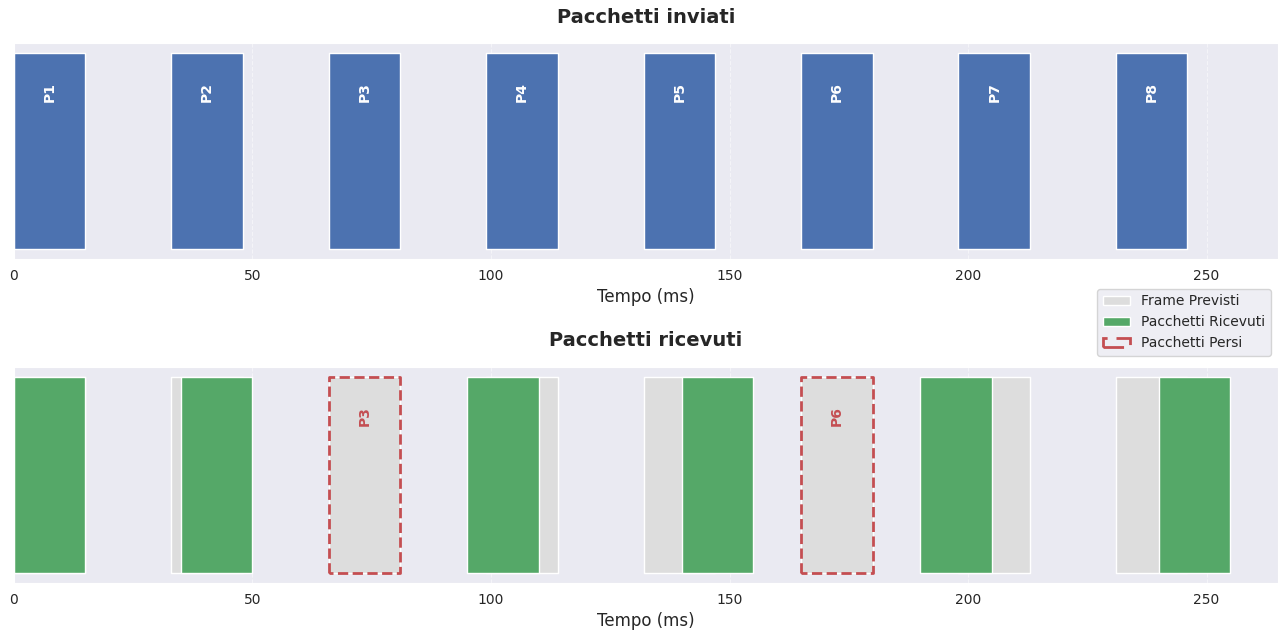
\includegraphics[width=0.9\textwidth]{figures/jitter.png}
    \caption{Effetto del jitter nella riproduzione dello streaming. Senza buffering i pacchetti non vengono riprodotti seguendo la stessa temporizzazione della sorgente.}
    \label{fig:jitter}
\end{figure}

Esistono 2 principali tipologie di software in questo contesto: interattivi (video-conferenze) e passivi (live-streaming). Nel primo caso i requisiti sul ritardo
e sul jitter sono molto stringenti, per cui non si possono introdurre meccanismi pesanti di bufferizzazione, poiché compromettono irrimediabilmente la user experience. Possono invece essere implementati nel secondo, in modo tale da mitigare gli effetti della trasmissione. Bisogna ridurre al minimo i tempi di attesa: ad esempio il reinvio dei pacchetti, come succede in TCP, non può essere implementato. UDP invece si presta a questo meccanismo ed infatti fornisce la base per un protocollo di streaming in tempo reale. Non instaura nessun tipo di connessione e non deve monitorare le condizioni della rete per adattare la sua velocità nella comunicazione. Real-time Transport Protocol(RTP) è un protocollo di livello trasporto\cite{a10rfc3550} %rfc3550 lo pone esattamente sul trasport layer("both protocols contribute parts of the transport protocol functionality") 
che è stato progettato per lavorare sopra UDP, e con le sue caratteristiche può soddisfare i requisiti per la trasmissione di dati multimediali su internet. RTP infatti permette la negoziazione di una codifica comune ai lati della comunicazione. Grazie a questo protocollo, i livelli applicativi sono liberi di implementare il buffering in base alle proprie necessità, poiché integra nei pacchetti il timestamp del contenuto multimediale. RTP non è sensibile al livello di congestione della rete, quindi il rate di trasmissione non viene modificato, come invece succede in TCP. %Si può tuttavia operare sul jitter, tramite riordinamento e buffering: se la variabilità nell'arrivo dei pacchetti porta ad una trasmissione fuori ordine, è possibile grazie alla bufferizzazione, a livello applicativo, risolvere questo problema. Inoltre, sempre grazie a questo meccanismo, si possono riprodurre i dati secondo il loro naturale timestamp, proprio perché questa informazione viene codificata nel protocollo di fatto utilizzato per le trasmissioni streaming in internet: Real-time Transport Protocol (RTP). 2. c'è da parlare anche del fatto che lo scarto di alcuni pacchetti non porta al degrado totale della user experience, ma in base allo use case e allo stato della rete si possono in qualche modo saltare dei pacchetti (un po' emerge quando si parla di sequence number).

RTP lavora in coppia con Real-time Control Protocol (RTCP), la sua controparte per la verifica dello stato della rete. A differenza di TCP, questo meccanismo ha una funzione di solo monitoraggio, non serve per reagire alle congestioni, quindi ai ritardi, alle perdite o al jitter. Si tratta di un protocollo leggero, che periodicamente invia messaggi di controllo verificando lo stato della rete. In questo modo i livelli applicativi, in base alla qualità che vogliono fornire, sono programmati per reagire di conseguenza. Si è delegato quindi al software questo onere, senza fornire una maniera standard per il controllo del traffico. Questo è un grosso vantaggio in termini di flessibilità: sfruttando TCP, al contrario, la velocità di trasmissione dipenderebbe dalle sue regole nel controllo del flusso di informazioni. Esiste infine un protocollo di più alto livello per la gestione delle sessioni nella trasmissione dati: Real-time Streaming Protocol (RTSP). Esso non inoltra i pacchetti effettivi per lo streaming, perché svolto interamente da RTP, ma una volta che la sessione è attiva, serve per inviare i comandi relativi allo stato di quest'ultima. Per cui il client che richiede dati multimediali manderà al server dei messaggi per avviare, sospendere o fermare il flusso di informazioni.

%rtp: protocollo di trasporto dati
%rtcp: protocollo di controllo di stato dello streaming
%rtsp: protocollo di controllo della SESSIONE di streaming 

\begin{figure}[htbp]
    \centering
    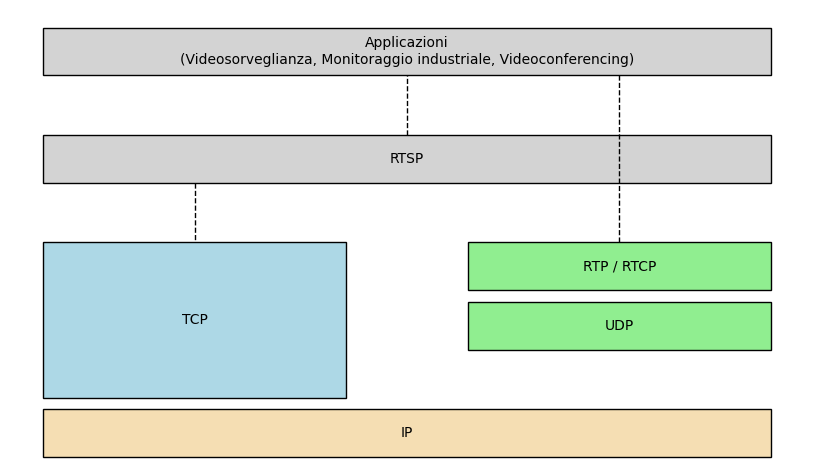
\includegraphics[width=0.8\textwidth]{figures/streaming_stack.png}
    \caption{Stack di protocolli per lo streaming real-time.}
    \label{straming-stack}
\end{figure}

Il formato dell'header RTP è costituito da tre elementi principali. I primi 12 bytes sono sempre presenti e formano il core del pacchetto. Successivamente possono esserci delle estensioni (anche se usate molto raramente) ed infine c'è il campo payload, il cui formato è deciso dall'applicazione. Nel dettaglio i campi di RTP sono:

\begin{itemize}
	\item \textbf{version}: bit per l'identificazione della versione di RTP usata nella trasmissione. 
	\item \textbf{padding}: se questo campo è configurato, sarà presente del padding nel pacchetto, ad esempio per allineamento oppure se si sta utilizzando qualche algoritmo di cifratura. 
	\item \textbf{extension}: quando il bit è attivo, il campo extension header viene collocato nel pacchetto. 
	\item \textbf{CSRC Count}: conta il numero di sorgenti multiple, quando sono presenti, come spiegato nel campo CSRC. 
	\item \textbf{marker}: identifica punti specifici nel flusso multimediale, come i confini tra diversi frame in un video.
	\item \textbf{payload type}: campo per la decodifica del contenuto multimediale nel payload.
	\item \textbf{sequence number}: numero identificativo del pacchetto. E' utile per stabilire se ci sia stata una perdita e permettere alle applicazioni di reagire. Queste possono decidere di non procedere in nessun modo oppure di attuare delle strategie. Ad esempio si potrebbe utilizzare delle codifiche che richiedono meno banda o riprodurre il frame precedente/successivo più volte.
	\item \textbf{timestamp}: indica il momento di generazione del pacchetto attraverso il clock di sistema. Serve per sincronizzare i flussi audio e video. Viene inoltre utilizzato per determinare il jitter.
	\item \textbf{Synchronization Source Identifier(SSRC)}: identifica la sorgente nella comunicazione RTP. E' un valore scelto randomicamente a livello locale dalle fonti, quindi esiste la possibilità di collisioni. In tal caso RTCP non permette che questo evento si verifichi, facendo uscire e rientrare dalla sessione una delle due sorgenti.
	\item \textbf{Contributing Source Identifiers(CSRC)}: è una lista delle sorgenti che contribuiscono al payload del pacchetto, anche se in generale il source è solitamente uno solo. E' utile nel caso delle videoconferenze quando più fonti generano un stream di dati, ma si vuole compattare i flussi in un unico pacchetto per necessità di banda. 
\end{itemize}

In RTP non è presente un concetto esplicito di sessione, ma esso viene definito contestualmente alla generazione dello streaming, identificando il destinatario tramite indirizzo IP e una coppia di porte RTP ed RTCP. %potrebbe aver senso parlare delle sessioni multimediali dove ad esempio viene gestito audio e video contemporaneamente. In quel caso si generano due flussi RTP e l'applicazione poi decide se usare entrambi i flussi o solo uno. In questo contesto si potrebbe introdurre il mixing. 

RTSP è nato come standard per la definizione delle sessioni multimediali ed il loro controllo. %nel caso di mqtt manca una trattazione approfondita della subscribe, qui manca per RTCP. 
In RFC2326 è definito come "remote control" nella gestione dello streaming, perché si presenta con una serie di comandi, che ricordano molto quelli di HTTP. Tuttavia differisce da questo protocollo in un punto fondamentale: RTSP è simmetrico, in quanto sia il client che il server multimediale possono inviare richieste. Inoltre i messaggi non sono di tipo fire and forget, infatti i comandi inviati possono riferirsi a richieste precedenti, rendendo di fatto RTSP un protocollo stateful\cite{a11rfc2326}. %specificare che gli stream vengono fatti su http, ma nel monitoraggio e nelle applicazioni industriali, dove i requisiti di latenza sono più bassi RTSP viene ancora utilizzato. Quale protocollo è più veloce tra RTP e WebRTC? 2. la simmetria di RTSP è specificata nel suo RFC. 3.segue qua sotto una cit da mio fratello in cristo durresi.
Non è un meccanismo orientato alle connessioni, per cui anche appoggiandosi a TCP potrebbe più volte aprire diverse comunicazioni attraverso lo stesso nella medesima sessione RTSP. In generale il suo funzionamento non dipende dal protocollo di livello 4 sottostante, per cui può servirsi sia di TCP che di UDP nella generazione dei propri messaggi, anche se di solito il primo è il più utilizzato. Nonostante i requisiti di bassa latenza per l'intero sistema di streaming, nel caso di RTSP è importante che i comandi arrivino a destinazione, per cui si utilizza un canale di comunicazione affidabile, separato dal flusso vero e proprio. Questo non comporta degrado delle prestazioni, perché la quantità di pacchetti è talmente limitata da non impattare sulla banda disponibile. Infine, per quanto riguarda le sue caratteristiche, bisogna menzionare come vengono identificati gli stream. 

Si sfrutta un RTSP URL, in maniera molto simile a come vengono definite le risorse in HTTP(e.g. \texttt{rtsp://hostname/video/front}). Questo mapping è molto utile perché si può applicare i comandi a più stream contemporaneamente, seguendo la gerarchia dei path nella stringa di identificazione. Ad esempio, se ci sono più flussi video, come \texttt{rtsp://hostname/video/front} e \texttt{rtsp://hostname/video/top}, per inviare un comando che si applichi ad entrambe le risorse, si sceglierà \sloppy\texttt{rtsp://hostname/factory/video}\fussy. %<---appendice dell'rfc
I metodi disponibili in RTSP sono:
\begin{itemize}
	\item \textbf{OPTIONS}: insieme dei comandi che entrambe le parti possono accettare; serve quindi per verificare la compatibilità delle operazioni disponibili tra gli estremi di comunicazione.
	\item \textbf{DESCRIBE}: questo comando fornisce la descrizione del contenuto multimediale come il formato e la codifica. 
	\item \textbf{SETUP}: inizializza la sessione di streaming RTSP, tramite dei parametri (e.g. porta, protocollo di trasporto) dopo che entrambe le parti hanno allocato le risorse necessarie.
	\item \textbf{PLAY}: il client invia questo comando quando richiede l'effettiva trasmissione del flusso.
	\item \textbf{PAUSE}: lo streaming viene interrotto dal client senza che il server liberi le risorse e i parametri di sessione.
	\item \textbf{TEARDOWN}: il client richiede lo stop dello streaming, seguito dalla liberazione delle risorse nel server.
	\item \textbf{GET\textunderscore PARAMETER, SET\textunderscore PARAMETER}: questa serie di comandi fornisce o imposta i parametri di sessione nello streaming (ad esempio i pacchetti ricevuti, il jitter etc). 
\end{itemize}

RTSP definisce una macchina a stati, che permette la coordinazione del flusso di streaming multimediale, in modo tale da consentire ai partecipanti della sessione di sapere quali comandi possono inviare o ricevere in ogni sua fase. Sia il client che il server memorizzano lo stato della sessione per avere una interazione coerente tra di loro. 

%cerca l'esempio di sessione per la generazione di un flusso infinito. nel caso mettilo qui ed aggiungi un grafico, oppure fallo in appendice. 

%l'introduzione al cloud fornita nel background non è formale ed è stata subito incentrata verso le nuove industrie. quindi puoi dare una definizione più rigorosa di cloud e di aws.
\section{Amazon Web Services}
%introduzione
Amazon Web Services (AWS) è una piattaforma pubblica basata su cloud che offre servizi gestiti per la generazione di soluzioni a diversi livelli di astrazione. Per quanto riguarda lo storage, ad esempio, si potrebbe richiedere al provider una macchina virtuale e collegare ad essa un volume, implementando così una soluzione di basso livello. Altrimenti è possibile sfruttare servizi come S3 e salvare le proprie informazioni attraverso una API, ottenendo un risultato simile, ma ad alto livello. La scelta dipende sempre dalle necessità dell'utente, tuttavia l'opzione più facile è sicuramente la seconda, perché, con una semplice chiamata, si possono salvare le proprie informazioni come se si utilizzasse un filesystem remoto, senza preoccuparsi della gestione interna, della durabilità, delle dimensioni dei file ed in generale della grandezza dello storage, che può scalare teoricamente in maniera indefinita. %livello piattaforma, livello servizi --> descrivi i modelli del cloud (saas,paas,iaas,haas).

Le API sono accessibili attraverso protocolli web, coerente con le caratteristiche fornite da NIST per quando riguarda il cloud computing. Tra queste, infatti, è presente il concetto di "broad network access", cioè le funzionalità del provider vengono erogate attraverso la rete. Altre proprietà comprendono: possibilità di ottenere i servizi su richiesta da parte dell'utente senza ausili esterni (on-demand self-service), condivisione di un'unica piattaforma per gli sviluppatori (resource pooling), risposta rapida alla richiesta di risorse imposte dalla variabilità nel workload (rapid elasticity).  
%geolocalizazione e modello di pagamento.
%benefici
L'adozione del cloud computing viene spesso sponsorizzata per il modello dei costi, basata sul pay-per-use. Questo significa ridurre le spese nel caso di startup che non possiedono una infrastruttura IT, oppure per aziende che vogliono ricostruire o estendere la propria. Inizialmente può essere un vantaggio, ma bisogna sempre monitorare l'utilizzo e l'archiettura delle proprie soluzioni in modo che i costi operativi non esplodano. In generale quindi il modello introdotto da Amazon può essere considerato un beneficio, tuttavia si tratta del punto di partenza per esplorare ulteriori vantaggi che il provider introduce. 

%1. innovation and integration
AWS è una piattaforma innovativa, che annuncia costantemente nuovi prodotti. L'implentazione di queste tecnologie viene poi integrata nell'ecosistema, contribuendo al suo continuo allargamento. %2. common problem resolution
I servizi gestiti forniti dal provider sono pensati per risolvere problemi comuni, in modo tale che il cliente si focalizzi solo sulle soluzioni. Per cui non sarà necessario implementare meccanismi di load balancing o per le notifiche in quanto AWS fornisce queste funzionalità a priori. %3 automation
Il paradigma Infrastructure as Code (IaC) rende la gestione delle risorse automatica: si tratta di un effetto collaterale dell'utilizzo delle API. L'utente deve solo dichiarare gli elementi necessari, non gestire manualmente la loro allocazione. Una volta definite le parti del sistema, sarà compito di AWS invocare i comandi che servono per la loro creazione. %4 scaling
La capacità del cloud si può adattare in proporzione al carico di lavoro, definendo un numero di macchine virtuali in base alla periodicità (giorni, settimane, mesi) e a quando vengono raggiunti i picchi. Basta incrementare il numero di risorse e quando non saranno più necessarie eliminarle. Questo meccanismo avviene molto velocemente, quindi non si tratta solo di un vantaggio di scalabilità, ma anche di velocità di allocazione e deallocazione delle risorse. %5 relability
AWS offre dei servizi che sono affidabili by default: ad esempio S3 è progettato per avere una durabilità dei dati al 99,9\%. Inoltre vengono forniti strumenti perché questo principio sia implementato a livello di sistema, non limitandosi quindi solo ai servizi. La possibilità di poter deployare la propria infrastruttura in più regioni rientra in questa categoria. Oltre ad essere un vantaggio in termini di accessibilità, latenza e protezione dei dati, quando una delle repliche possiede un guasto, si può continuare a garantire il servizio utilizzando il deploy di un'altra regione. Inoltre, sempre nell'ottica dell'affidabilità, vengono forniti dei moduli per il monitoraggio e l'alerting dell'infrastruttura, come nel caso di Amazon CloudWatch e AWS X-Ray. Si possono così controllare le metriche principali come latenza, utilizzo delle risorse e throughput. Nel momento in cui si verificano anomalie è possibile infine impostare degli avvisi per reagire tempestivamente agli eventi inattesi. 

%introduzione ai servizi e deep-down a quelli che ho utilizzato
Come si può notare in Figura \ref{fig:services_taxonomy}, i servizi offerti da AWS si dividono in due categorie: hardware e software, basati sull' infrastruttura sottostante\cite{a12AWSinAction}. Poiché in questo lavoro si è sfruttato unicamente il modelli Platform as a Services (PaaS) e Software as a Service (SaaS), 
il focus della classificazione nell'analisi sarà solo sulla parte software.
%vedi se riesci a produrre un'immagine coerente
\begin{figure}[htbp]
    \centering
    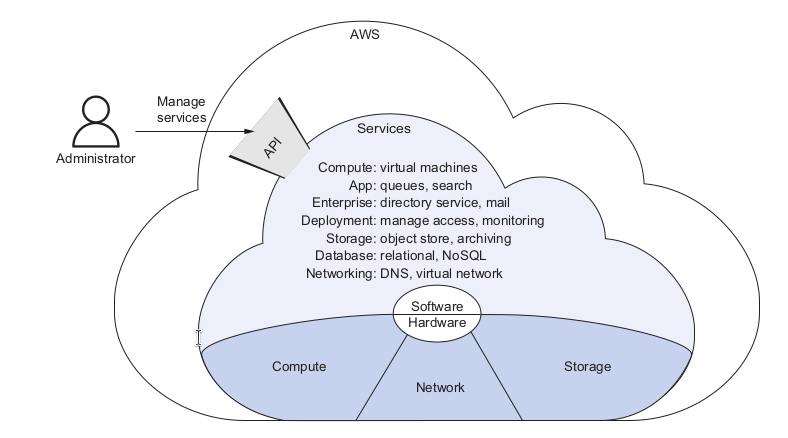
\includegraphics[width=0.59\textwidth]{figures/aws_services_taxonomy.png}
    \caption{Classificazione ad alto livello dei servizi AWS. Accessibili attraverso API, si dividono nelle due macro-aree hardware e software.}
    \label{fig:services_taxonomy}
\end{figure}

Per quanto riguarda la categoria compute, l'obiettivo è quello di fornire rispettivamente servizi per l'esecuzione di applicazioni su macchine virtuali e per la gestione delle risorse di calcolo, come nel caso di Elastic Compute Cloud (EC2). Per app si intendono quei servizi a diretto supporto delle applicazioni, necessari per la risoluzione di problemi comuni, come l'implementazione delle code di messaggi o delle notifiche. I servizi enterprise sono pensati per la gestione delle risorse aziendali, ad esempio Organizations è un tool per il controllo di più account AWS, in modo tale da poter effettuare raggruppamenti in base alle unità nell'organizzazione ed aggregare policy e operazioni per ciascun gruppo. La categoria deployment, come si può facilmente intuire, fornisce strumenti per la distribuzione del software. Storage è l'insieme dei servizi per la memorizzazione dei dati in modo sicuro, scalabile e di lunga durata. Tra questi rientrano sicuramente gli object store come S3 e i servizi di archiviazione a lungo termine e backup come Glacier. Le ultime due categorie riguardano i database (RDS per i relazionali, DynamoDB per quelli non relazionali) ed il networking come Virtual Private Cloud (VPC) per la creazione di reti isolate nella piattaforma. %mancano networking e database.
In Tabella \ref{tab:aws_services}, infine, viene mostrata la tassonomia, secondo le classi appena definite, dei servizi usati nell'implementazione del sistema di rilevazione dei DPI, con una breve descrizione del loro funzionamento, reperibile dettagliatamente dalla documentazione Amazon\cite{a13AWSDoc}. 

\begin{longtable}{@{}p{3cm}p{2.5cm}p{7cm}@{}}
\toprule
\textbf{Servizio} & \textbf{Categoria} & \textbf{Descrizione} \\ \midrule
\endfirsthead

\endhead
%\bottomrule
%\endfoot

%\toprule
CloudFormation & Deployment & Tramite il paradigma Infrastructure as Code, permette la dichiarazione di uno stack con le risorse necessarie ed indica le policy di accesso tra i vari servizi. \\ \midrule
Lambda & Compute & Funzione utilizzata in architetture event-driven, programmata senza dover gestire l'infrastruttura sottostante (macchine virtuali, sistemi operativi). \\ \midrule
IAM Policy & Enterprise & Consente di definire le regole di accesso e autorizzazione tra servizi AWS, rendendo possibili interazioni sicure e controllate. \\ \midrule
Kinesis-Video Streams & App & Gestisce in maniera scalabile l'ingestion di flussi multimediali dall'esterno del cloud e li inoltra a servizi downstream, come S3, EC2 o applicazioni di machine learning (e.g. Rekognition). \\ \midrule
Kinesis-Data Streams & App & Progettato per gestire flussi di dati non multimediali (JSON, testo), provenienti da fonti come sensori IoT, inoltrati successivamente a servizi big data come Kinesis Data Analytics(KDA) o per lo storage (S3, DynamoDB). \\ \midrule   
Kinesis-Data Analytics & App & Utilizzato per analisi dei dati in real-time, provenienti da flussi generati da Kinesis Data Streams oppure Apache Kafka. \\ \midrule
Amazon Rekognition & App & Sfrutta modelli di Deep Learning per identificare oggetti, persone, scene all'interno di immagini e video. \\ \midrule
AWS IoT Core e Greengrass & App & Controllano in maniera coordinata lo stato dei dispositivi IoT e inoltrano i relativi messaggi di telemetria provenienti dall'edge. \\ \bottomrule
\caption{Classificazione dei servizi AWS di interesse.} \label{tab:aws_services}
\end{longtable}

Fatta eccezione per Amazon Rekognition, tutti questi servizi rientrano nella categoria PaaS, in quanto gran parte della gestione è delegata ad AWS, ma sono necessarie delle ulteriori configurazioni perché possano funzionare correttamente. Ad esempio Kinesis Data Analytics richiede di sviluppare applicazioni come Apache Flink e di collegare sorgenti e destinazioni. %Come già visto nel precedente capitolo invece, per usare Amazon Rekognition basta invocare la sua API e si otterrà subito una risposta, senza ulteriore overhead di gestione. 
%aggiungi tabella con i servizi che hai usato
% Si descriverà in dettaglio il servizio Amazon Rekognition, sottolineando le sue capacità di analisi delle immagini e dei video attraverso algoritmi di deep learning. Si spiegherà come il servizio possa essere utilizzato per il riconoscimento di oggetti, volti e scene, e perché è particolarmente adatto per il rilevamento dei DPI.
%Vedi se piazzare questa parte nelle tecnologie. dipenderà molto da come affronterai la parte relativa ai lavori simili.

AWS possiede un ricco ecosistema per la generazione di soluzioni basate sull'apprendimento automatico, tra cui, oltre a Rekognition, SageMaker e Bedrock. Ciascuno risponde a esigenze specifiche: SageMaker funge da piattaforma di base per lo sviluppo e l'addestramento di modelli personalizzati, mentre Bedrock offre accesso a diversi foundation models, semplificando l'utilizzo di questa nuova tecnologia. Infine, Rekognition si posiziona come una soluzione specializzata per l’analisi di immagini, video e streaming, dove le aziende possono implementare le relative funzionalità senza dover sviluppare o addestrare modelli. Serve solo invocare la API di interesse. Rekognition è quindi particolarmente utile alle compagnie che necessitano di integrazioni rapide e affidabili nell'ambito della visione artificiale all'interno dei loro processi. I casi d'uso spaziano su numerosi domini: ad esempio, può essere utilizzato per estrarre metadati da un testo scritto a mano, oppure per la moderazione dei contenuti nelle piattaforme social.

\begin{figure}[htbp]
    \centering
    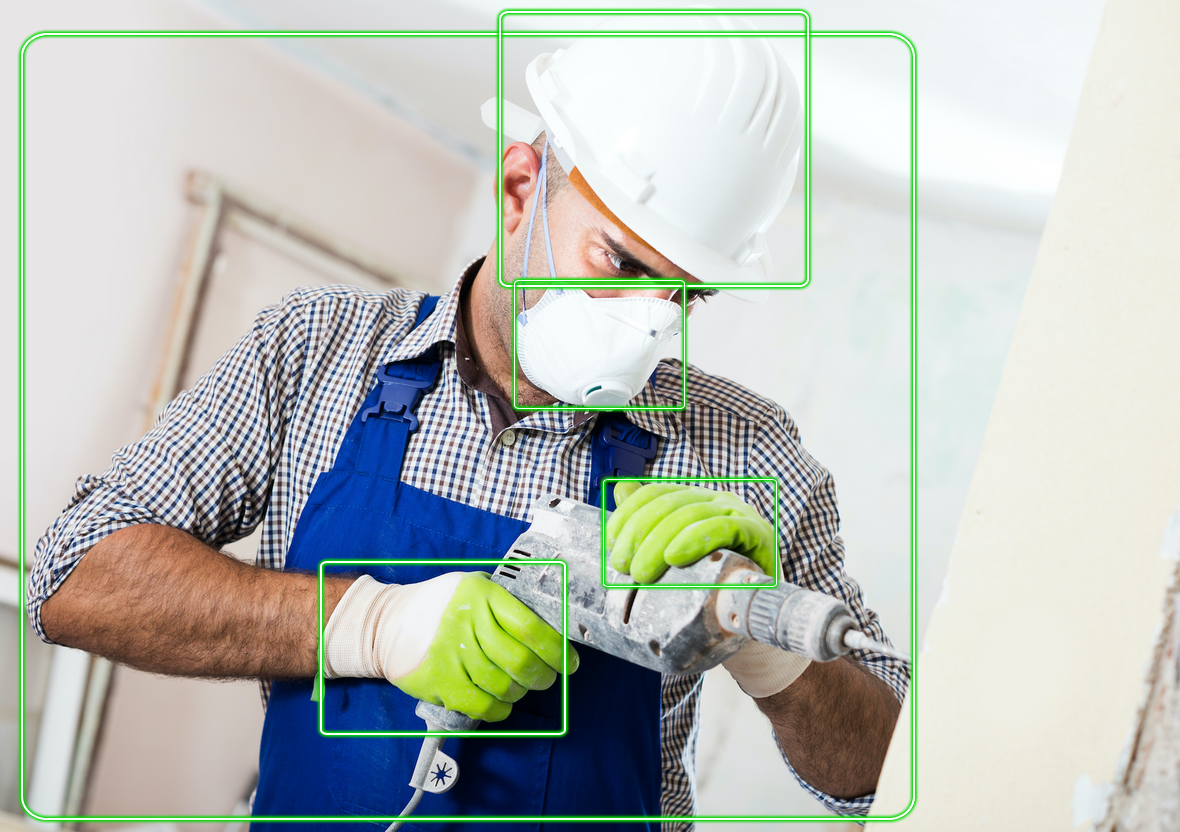
\includegraphics[width=0.59\textwidth]{figures/worker-with-bb.png}
    \caption{Rilevamento tramite Rekognition dei dispositivi di sicurezza individuali.}
    \label{fig:ppe-example}
\end{figure}


\noindent Nell'ambito di questo scritto, Rekognition viene usato per l'identificazione dei dispositivi di sicurezza e per la valutazione del loro corretto utilizzo. Dalla documentazione Amazon viene mostrato un esempio di questo servizio in azione. La API utilizzata è DetecProtectiveEquipment, che in questo caso è in grado di rilevare casco, maschera e guanti da lavoro. Più nel dettaglio, la risposta di questa richiesta sarà una struttura dati contenente: le persone all'interno dell'immagine, le parti del corpo che indossano i dispositivi di sicurezza (differenziando ad esempio quale mano indossa i guanti), il tipo di dispositivi rilevati e l'associazione tra parti del corpo e dispositivi, in modo tale da verificare quali siano correttamente indossati. La chiamata può essere configurata per rilevare tutti i DPI più comuni oppure solo un sottoinsieme di essi, in base alla necessità. Le API di Rekognition si differenziano in due possibili sottocategorie: storage e non-storage. La distinzione consiste nel fatto che il servizio può salvare o meno le informazioni relative all'analisi dell'immagine o del video. Per questioni di privacy, non viene tracciato alcun individuo e non c'è alcuna correlazione tra gli id restituiti da ciascun processamento. L'operazione è focalizzata solo sull'utilizzo regolare dei DPI e la documentazione è molto attenta su questo tema. Altre chiamate di Rekognition, come quelle basate sul riconoscimento facciale, hanno invece bisogno di salvare queste informazioni, altrimenti non potrebbero funzionare.

%\subsection{Infrastructure as Code}
%\subsection{Serverless}
%\subsection{Iam Policy}
%\subsection{Kinesis Video Streams}
%\subsection{AWS Iot Core e Greengrass}
\section{Apache Flink}

Apache Flink è un framework open source, nato per l'elaborazione intensiva dello streaming di dati in real-time. Le sue performance sono dovute a come questa tecnologia è stata pensata. In primo luogo, a differenza delle architetture applicative tradizionali, i software basati su Flink non condividono lo stato esternamente, risolvendo vincoli di scalabilità ed efficienza man mano che i software evolvono. Nei sistemi transazionali, in cui molti applicativi si basano sulla stesso database, una piccola modifica al modello dei dati può causare molti problemi, se non si opera con la massima accuratezza. Una soluzione è stata quella di introdurre l'architettura a microservizi, dove vengono esposte interfacce REST al posto delle chiamate dirette alla base dati. Nei sistemi di data analysis invece, come quelli basati su data warehouse, sono presenti limitazioni a livello di sincronizzazione e di complessità di trasformazione, in quanto i dati devono essere periodicamente estratti da diverse sorgenti per essere centralizzati in un unico punto. Il secondo elemento importante nel design di Apache Flink, strettamente correlato al primo, è lo snapshot dello stato, ovvero un meccanismo per recuperare dai guasti. Questo è fondamentale, in quanto il framework è un sistema distribuito e può essere soggetto a failure, come errori interni ai nodi, eccezioni o problemi di connettività. La garanzia che lo stato non venga perso, avviene tramite il checkpointing, cioè il salvataggio dei dati in un store remoto. Non si tratta solamente di un metodo di prevenzione, ma un elemento critico per il funzionamento del sistema. In Apache Flink, senza questa garanzia, nessuna applicazione sarebbe in grado di operare in maniera coerente, perché molto spesso i dati vengono elaborati sfruttando delle finestre di aggregazione. Durante questi intervalli, potenzialmente molto lunghi, potrebbero verificarsi delle inconsistenze. Nell'elaborazione non è importante solamente il concetto di stato, ma soprattutto quello di stream. E' difficile nel mondo reale trovare domini in cui tutti i dati vengono generati in un colpo solo. La loro creazione è piuttosto l' effetto di un costante flusso di eventi, ad esempio attraverso l'interazione utente su interfacce web e applicazioni mobili, oppure dalle informazioni provenienti dai dispositivi IoT \cite{a14Flink}.
Sintetizzando le idee di flusso e di stato, si ottiene il pattern fondamentale su cui è basato Apache Flink: Stateful Stream Processing. L'ultimo elemento core del framework è il concetto di event time, ma nel contesto di questo elaborato resta marginale, in quanto non è stato sfruttato nello sviluppo del sistema. %vedi come estendere qui.
Esistono infatti due modalità in cui i dati possono essere processati, di cui il più semplice è il processing time. L'applicazione, seguendo questo paradigma, esegue le elaborazioni in base al clock del sistema piuttosto che basarsi sul timestamp degli eventi. Event time processing è un meccanismo utilizzato nel caso in cui ci sia una necessità di ordinamento tra i record in ingresso, ma nel prototipo costruito non è fondamentale, in quanto è necessario solo capire se dato un certo numero di risultati provenienti dall'analisi del modello di machine learning, questi globalmente superino una certa soglia, senza alcun vincolo nella loro disposizione.

%definizione di streaming e differenze tra frameworks big data
Il tipo di processamento in Flink non è indirizzato solo verso i flussi di dati, ma anche al batch, che può essere visto come un caso limite di stream processing. In particolare, il numero di elementi in ingresso può essere di due tipologie: limitato o illimitato. Nel secondo caso le informazioni vengono raccolte e successivamente elaborate in blocco. Così Flink, pur essendo un framework nativamente pensato per lo streaming, offre molta flessibilità, grazie a più modalità di computazione disponibili. In generale nel panorama big data non è lo standard, infatti Apache Spark permette di elaborare grosse quantità di dati, ma con una latenza maggiore, perché non è nativamente progettato per lo streaming. E' altrettanto vero che sono stati introdotti meccanismi per superare queste limitazioni, come il supporto al micro-batching, ma non riesce comunque a raggiungere le stesse performance per questo tipo di applicazioni. Nella modellazione del flussi, viene utilizzato il concetto di dataflow graph, composto da una sorgente, degli operatori ed infine un collettore (sink). Questo tipo di rappresentazione segue una struttura DAG (Direct Acyclic Graph) ed è fondamentale per il framework, in quanto il codice fornito all'applicazione passa per diverse rappresentazioni ed ottimizzazioni intermedie. Nel dettaglio, una prima versione logica del grafo viene creata a partire dall'applicativo. Successivamente si passa a quella fisica, ed infine si arriva all'esecuzione. L'architettura di Apache Flink è composta ad alto livello da tre componenti: il client, quindi il codice scritto dallo sviluppatore, il Job Manager ed infine il Task Manager.  Il Job Manager riceve dall'applicazione il grafo di più alto livello e si occupa dell'allocazione delle risorse nell'infrastruttura di deployment. Nella pratica, vengono attivate una serie di Task Manager, in modo tale da dividere il job in diverse elaborazioni parallele. Questo implica sia una suddivisione delle risorse computazionali che un partizionamento dei dati. 

\begin{figure}[htbp]
    \centering
    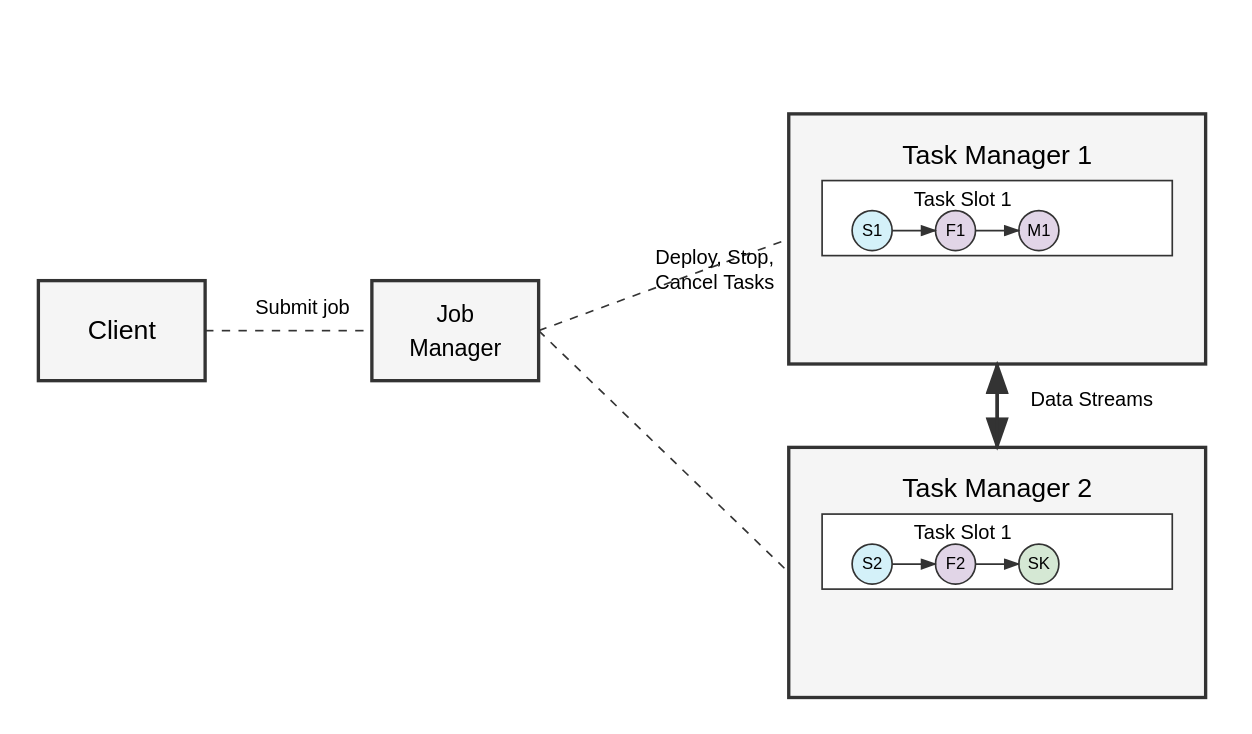
\includegraphics[width=0.8\textwidth]{figures/flink-architecture-simple-final.png}
    \caption{Esempio di funzionamento del runtime in Apache Flink.}
    \label{fig:flink-arch}
\end{figure}

Come si può notare in Figura \ref{fig:flink-arch}, ogni Task Manager fornisce una serie di task slots, ciascuno dei quali può eseguire una istanza parallela di un grafo. Una volta che il job viene lanciato, il Job Manager rimane responsabile del coordinamento delle attività nel cluster, ad esempio riavvia i Task Manager quando falliscono. Questi ultimi, una volta lanciato un job, prendono i dati da source differenti, li trasformano e, prima di caricarli sul sink, possono reciprocamente inviarsi le informazioni. 
Ciò avviene per mezzo di strategie, che definiscono come i dati vengono scambiati in un dataflow graph fisico. Possono essere automaticamente invocate dal framework, oppure possono essere esplicitamente dichiarate in fase di scrittura del codice. I pattern principali sono i seguenti:

\begin{itemize}
	\item \textbf{forward}: permette di portare gli elementi dalla sorgente ad un altro punto del grafo. E' l'operazione più semplice e meno costosa che si possa applicare.
	\item \textbf{repartition}: si tratta di un'operazione di filtro e raggruppamento. Questo tipo di operazione è più costosa del forward. I dati devono essere serializzati, perché in base a qual è l'operatore di destinazione, potrebbero essere spediti in rete. Un altro operatore infatti potrebbe trovarsi su un nodo diverso da quello di partenza.
	\item \textbf{rebalance}: questa operazione riduce il parallelismo dello stream, ad esempio si potrebbe passare da due flussi ad uno solo. Per l'arbitraggio dei dati che attraversano l'operatore si sfrutta l'algoritmo Round-Robin. Anche in questo caso il costo dell'operazione è rilevante, in quanto di nuovo è necessaria la serializzazione e l'invio in un altro nodo dell'infrastruttura.
\end{itemize}  

In Figura \ref{fig:dataflow-l} viene mostrato un esempio di dataflow logico, con diverse trasformazioni. Il source può essere di varie tipologie e, nell'ambito di questa tesi, viene utilizzato il Kinesis Data Stream connector, per estrarre i record dal servizio gestito Amazon. %fornisci un esempio e aggiungi un commento per le trasformazioni che salvano internamente lo stato.

\begin{figure}[htbp]
    \centering
    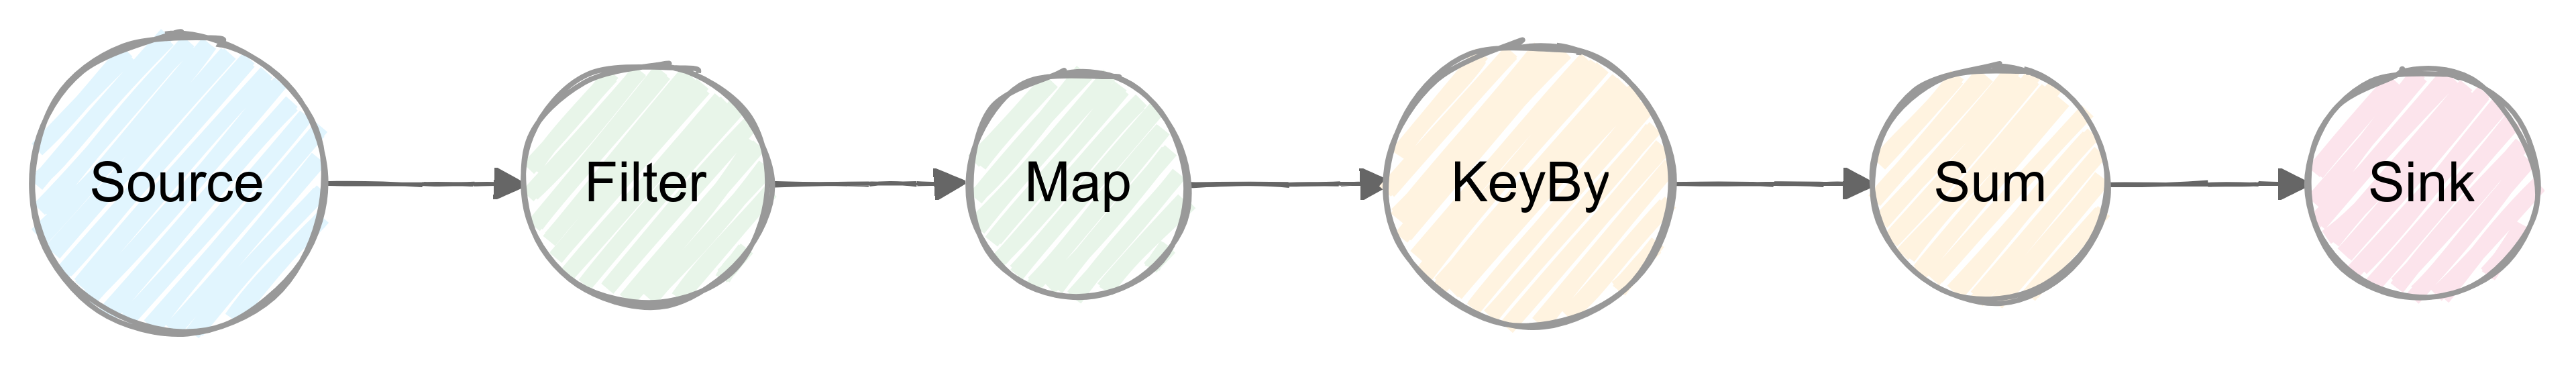
\includegraphics[width=0.7\textwidth]{figures/logical-dag.png}
    \caption{Dataflow livello logico.}
    \label{fig:dataflow-l}
\end{figure}  

Questo grafo viene elaborato dal Job Manager, subendo una mappatura nel cluster, come descritto precedentemente nell'architettura del runtime di Flink. In Figura \ref{fig:dataflow-phy} si può notare come alcune trasformazioni sfruttino intrinsecamente i pattern appena descritti. %aggiungi magari esempio numerico, e specifica che questo a tutti gli effetti è un esmepio di stateful stream processing
Un altro dettaglio, che non viene mostrato nella rappresentazione del dataflow fisico, è il salvataggio dello stato. Ciascun operatore stateful, come le operazioni di aggregazione, basate su una chiave di raggruppamento, può infatti persistere localmente informazioni associate a più elementi processati nel tempo. %espandi questa parte, mostrando che viene implementato proprio a questo livello il concetto di snapshot. 


\begin{figure}[htbp]
    \centering
    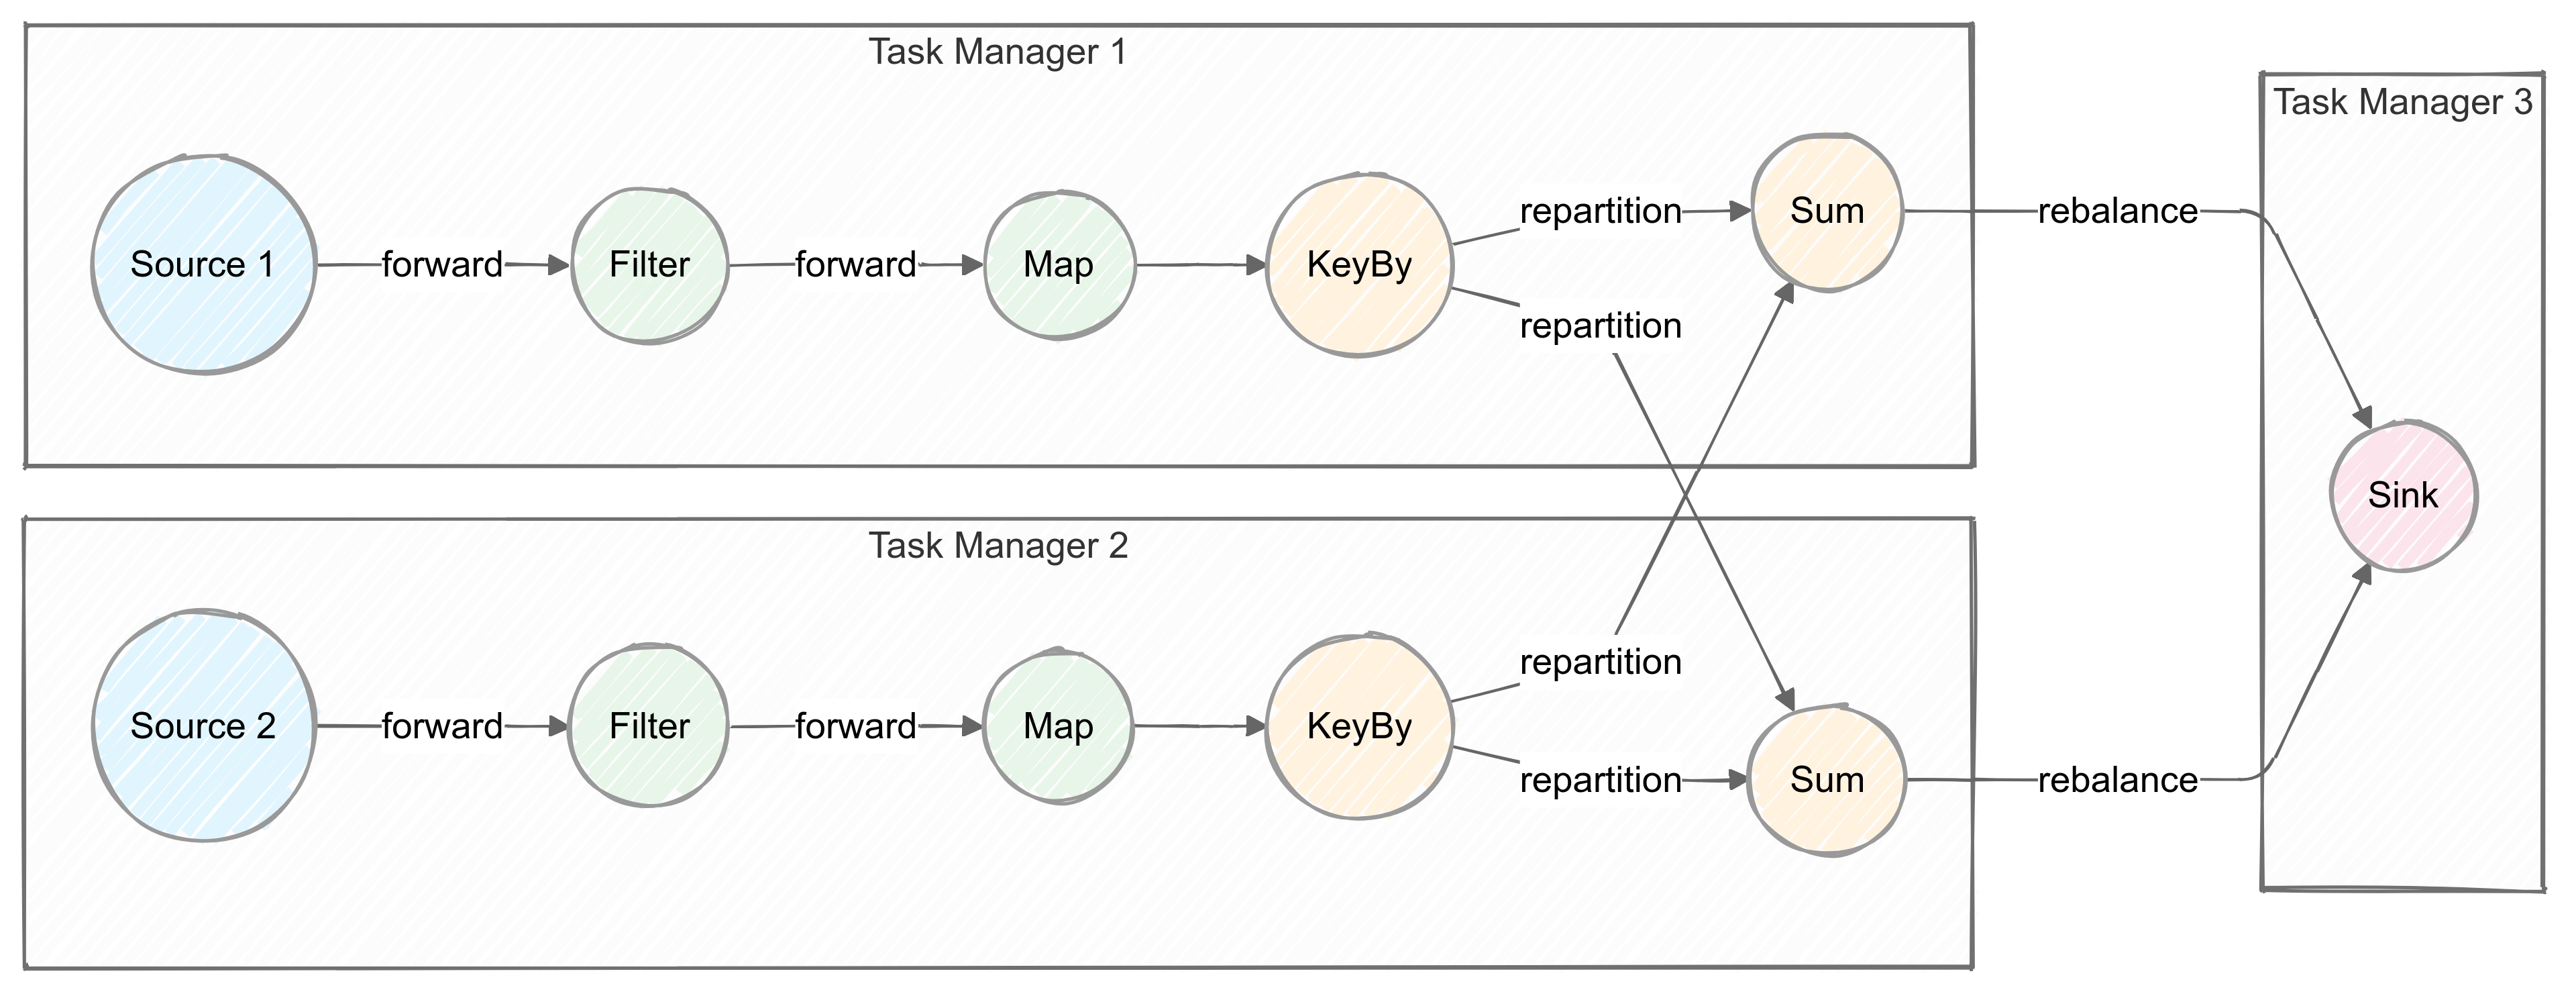
\includegraphics[width=0.7\textwidth]{figures/physical-dataflow-example.png}
    \caption{Dataflow livello fisico.}
    \label{fig:dataflow-phy}
\end{figure}  


Il dataflow logico è generato a partire da Datastream API, una delle interfacce possibili fornite dal framework. Apache Flink offre chiamate a diversi livelli di astrazione, in base al tipo di necessità dello sviluppatore. L'insieme di API di più basso livello nello stack è costituito da process functions e Datastream. Le prime possono implementare qualsiasi operazione, manipolando direttamente lo stato e i timers. Queste primitive in realtà vengono usate in coppia con Datastram, in quanto le API in Apache Flink non sono esclusive, ma interoperabili. Quindi, dal punto di vista implementativo c'è molta flessibilità, perché nel caso di richieste specifiche nella gestione degli stream, si può passare a chiamate di più basso livello, come nel caso dei timer, che servono per la gestione delle finestre temporali. Idealmente, si vorrebbe salvare sempre lo stato nelle operazioni stateful, ma questo comporta dei problemi in termini di risorse. Il flusso di dati, come già visto, è indefinito, quindi l'unica soluzione per poter mantenere uno stato di dimensioni accettabili è quello di effettuare le elaborazioni per un numero di eventi limitato. L'utilizzo delle finestre serve esattamente per questo tipo di scenario. Nell'implementazione del sistema sono state usate due tipologie di aggregatori: quelle basate sulla sul conteggio (count windows) e quelle su timer (time windows). %espandi questa parte per concludere
%dove viene salvato lo stato
%tipologie di source
%altri pattern: broadcast -> distribuisce i dati sul cluster, join -> data enrichment

%nota dall'esempio che la proprietà di DAG è mantenuta.
%datastream api
%finestre
%flink SQL è una delle api disponibili agli sviluppatori. Le altre api operano a livelli inferiori di astrazione. 
% process functions(bottom): primitive che possono implementare praticamente qualsiasi operazione manipolando direttamente lo stato in flink e i timers. A questo livello il codice scritto reagisce a qualasisi evento quando arriva, ogni volta. Queste funzioni in realtà fanno parte della 
%DataStream API: ci troviamo ad un livello di astrazione leggermente più alto, dove i building block includono stream e finestre. (r: chissà come vengono implementati gli stream con solo le primitive).Table API: è praticamente equivalente a flink SQL, ma a questo livello, piuttosto che scrivere direttamente sql si sta scrivendo il codice in java, o python.

 
%opzionale: ai livelli di astrazione crescenti, non corrisponde la stessa strtificazione del codice nell'implementazione. Le process functions sono parte di datastream API. Flink SQL e table api sono due facce della stessa medaglia. La table api non è implementata sopra la datastream API. Entrambi i blocchi sono implementati sullo stesso basso livello interno (stream operator api). 


%Stafeful stream processing
     
%\section{GStreamer}



